\chapter{Suites numériques}

\label{chap:suite}
\section{Introduction~: Une histoire de flocons}
On s'intéresse à mesurer le périmètre d'un flocon de neige. Pour y arriver, on a l'idée de partir d'un polygone simple, un triangle équilatéral, et de construire un flocon étape par étape. Pour construire le polygone de l'étape suivante, on procède comme suit:
\begin{enumerate}
    \item On divise chaque segment du polygone en 3 parties égales
    \item On ajoute un triangle équilatéral qui a comme base le tiers du milieu
    \item On efface la base de ce dernier triangle
\end{enumerate}
Ce procédé est illustré dans l'image suivante:
\begin{figure}[H]
\centering 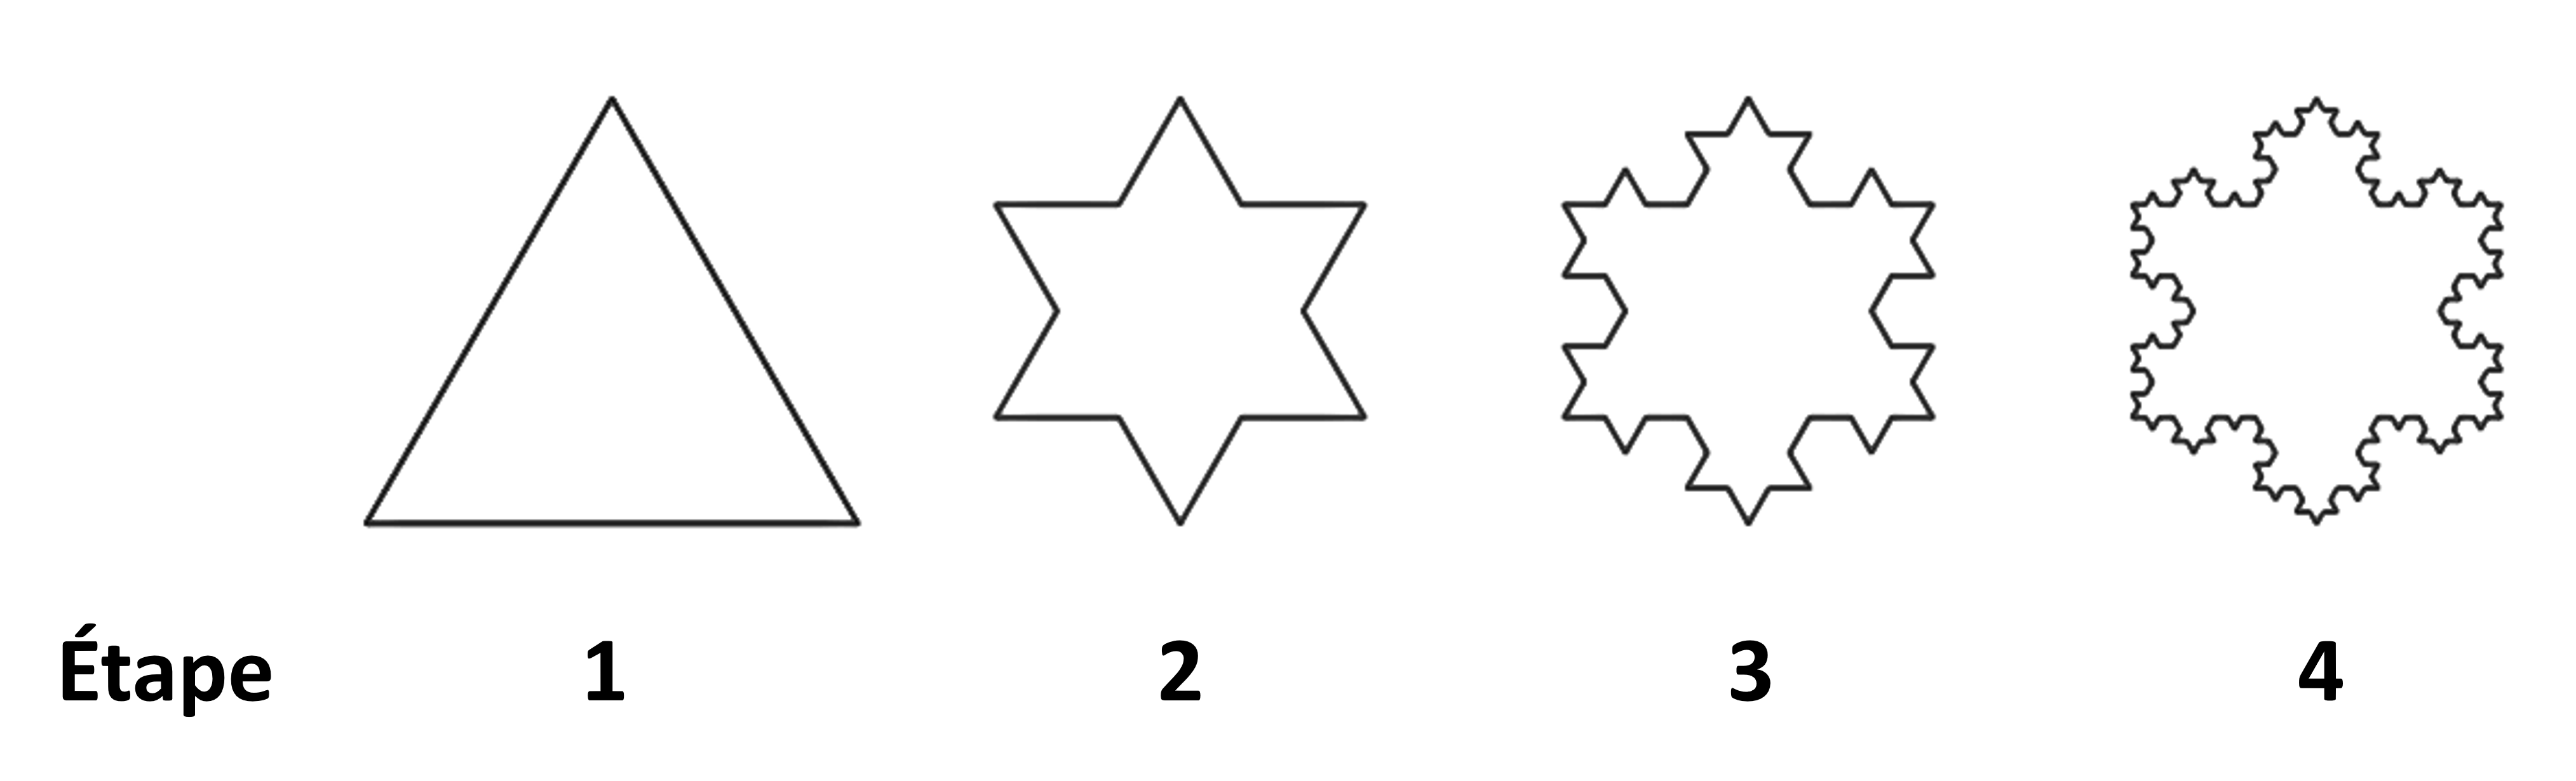
\includegraphics[width = 0.85\textwidth]{./assets/imgs/Koch-snowflake.png}
\caption{Les 4 premières étapes dans la construction du flocon de Koch}
\label{fig:koch}
\end{figure}
En supposant que chaque côté du triangle initial a une longueur $l$, le périmètre à la première étape vaut $3\times l$. D'une étape à l'autre, chaque segment passe d'une certaine longueur $d$, à une longueur $2\times d/3 + 2\times d/3 = 4d/3$, car on a transformé 3 tiers en 4 en ajoutant le triangle équilatéral et en en enlevant la base. 

Tout ceci nous permet de définir une suite $(p_n)_{n\in \mathbb N^*}$, qui, pour chaque nombre entier $n$, nous donne le périmètre du polygone obtenu en appliquant $n-1$ fois le procédé décrit plus haut, autrement dit:
\begin{equation}
    p_{n+1} = p_n\times \frac{4}{3} \label{eqn:koch}
\end{equation}

On peut écrire les premiers termes de la suite avec en plus la \emph{condition initiale} que $p_1= 3l$:

$$ p_1 = 3l \, , \,  p_2 = 3l \cdot \frac{4}{3} = 4l \, , \, p_3 = 4l \cdot \frac{4}{3} \, , \, \dots$$

Ceci nous motive à écrire la définition d'une suite suivante.

\begin{boxdef}[Suite]
Une telle séquence de nombres réels $p_1, p_2, p_3, ...$, indexée par les entiers positifs de $\mathbb N$, est appelée \emph{suite}. On la note $(p_n)_{n \in \mathbb{N}^*}$, $(p_n)_{n \geq 1}$, ou simplement $(p_n)$, et on note $p_n$ le $n$-ième élément de la suite.
\label{def:suite}
\end{boxdef}

Chose remarquable, on observe que le terme $p_{n+1}$ dépend des ternes précédents, ici c'est $p_n$.
 C'est un cas particulier d'une suite définie par \emph{récurrence}, c'est-à-dire que chaque terme nous est donné par une fonction des termes précédents de la suite.
En appliquant la formule (\ref{eqn:koch}) plusieurs fois, on peut obtenir (pour un $n>2$): 
\begin{equation}
    p_{n+1} = p_n\times \frac{4}{3} = p_{n-1}\times \frac{4}{3}\times \frac{4}{3} = \dots = p_1\times\left(\frac{4}{3}\right)^n
\end{equation}
On voit que pour ce type de suite particulière, appelé suite \emph{géométrique}, on a réussi à transformer la \emph{relation de récurrence}, en une relation qui ne dépend que du premier terme $p_1$ et de l'indice $n$. Ceci est très important, car pour étudier, par exemple, le périmètre à l'étape $n=43789$, je n'ai pas besoin d'avoir calculé les $43788$ périmètres précédents !

D'autres aspects intéressants de cette suite sont que, vu que $4/3 > 1$, on a que chaque terme est plus grand que le précédant, i.e. $p_{n+1} > p_n$, pour tous les indices $n$. Cette suite est dite \emph{strictement croissante}. On peut regarder le graphe pour s'en assurer :

\begin{figure}[H]
\centering 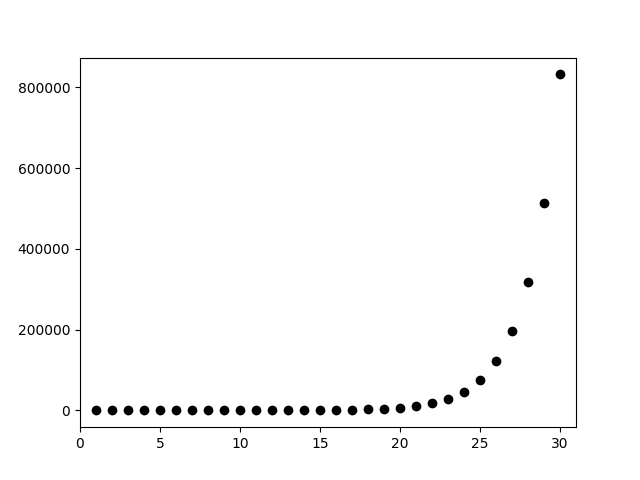
\includegraphics[width = 0.55\textwidth]{./assets/imgs/fibonacci.png}
\caption{Les 30 premières valeurs de la suite du périmètre du flocon de neige}
\label{fig:fibonacci}
\end{figure}

Les périmètres successifs n'arrêtent pas de monter, cela ne semble pas positif pour estimer le périmètre du flocon de Koch, qui correspond au périmètre obtenu après un nombre \emph{infini} d'étapes...
On peut donc dire que la suite $(p_n)$ n'est pas comprise entre deux valeurs fixes. Autrement dit, la suite $(p_n)$ n'est pas bornée.



\begin{boxdef}[Suite bornée et non-bornée]
Une suite $(x_n)$ est dite \emph{bornée} si on peut l'encadrer par deux valeurs fixes, i.e. s'il existe un nombre réel $B > 0$ tel que $-B < x_n < B$ pour \textbf{tous} les indices $n$ ! On dit que la suite est \emph{non-bornée} si un tel nombre $B > 0$ n'existe \textbf{pas}. De manière équivalente, une suite est non-bornée si pour tout $B > 0$, on peut trouver au moins un indice $n$ tel que $|x_n| > B$ (c'est-à-dire $x_n < - B$ ou bien $x_n > B$).
\label{def:borné}
\end{boxdef}


\section{Suites numériques}

Pour définir une suite, au sens de la Définition \ref{def:suite}, de manière rigoureuse, il y a 3 manières~:

\begin{enumerate}
    \item La suite est définie \emph{par récurrence}~: le $n$-ième élément $x_n$ est défini en fonction d'autres éléments $x_i$ avec des indices $i < n$. C'est le cas de la suite du flocon de Koch étudiée précédemment~: $p_{n+1} = p_n \cdot \frac{4}{3}$ pour $n \geq 1$ avec $p_1 = 3l$ comme point de départ. Il est important de bien donner les éléments initiaux de la suite, car ils ne peuvent pas être définis en termes d'autres éléments.
    \item La suite est définie explicitement~: le $n$-ième élément $x_n$ est une fonction de $n$. Par exemple, $x_n = n^2 + n - 2$ pour tout $n \geq 1$.
    \item La suite est définie par une propriété non-ambiguë~: par exemple, $x_n$ est le $n$-ième nombre premier.
\end{enumerate}

Les suites peuvent exhiber des propriétés diverses et variées. Il n'y a pas de règle générale permettant de décrire le comportement de toutes les suites en même temps. Certaines propriétés importantes permettent de les étudier plus en détails. Commençons par quelques exemples, suivis de définitions rigoureuses de ces propriétés~:
\begin{enumerate}
    \item La suite du flocon de Koch est croissante, non-bornée.
    \item La suite $x_n = (-1)^n$ est bornée, mais n'est ni croissante, ni décroissante. La suite alterne entre les valeurs $-1$ et $+1$.
    \item La suite $x_n = (-1)^n \cdot n$ est non-bornée, ni croissante, ni décroissante.
    \item La suite $x_n = \frac{1}{n}$ pour $n \geq 1$ est bornée car $-1 \leq x_n \leq 1$ pour tout $n \geq 1$, et elle est aussi décroissante.
\end{enumerate}
La première propriété importante est liée à la différence entre deux termes successifs, car elle nous permet en général de comprendre le comportement d'une suite lorsque $n$ devient grand sans en devoir calculer tous les termes.
\begin{boxdef}[Suite (strictement) croissante, décroissante]
Une suite $(x_n)$ est dite \emph{croissante} si pour \textbf{tous} les indices $n$, on a $x_{n+1}-x_n \geq 0$. Au contraire, une suite $(x_n)$ est dite \emph{décroissante} si pour \textbf{tous} les indices $n$, on a $x_{n+1}-x_n \leq 0$. Dans le cas où l'inégalité est stricte, la suite est dite \emph{strictement} croissante ou décroissante.
\label{def:croissante-decroissante}
\end{boxdef}
Le deuxième et le troisième exemple ne possèdent pas cette propriété, mais on peut les caractériser autrement! En effet, si on prend le deuxième exemple: $x_n = (-1)^n$, et que l'on construit deux autres suites $y_n = x_{2n} =(-1)^{2n} = ((-1)^{2})^n = 1$ et $z_n = x_{2n+1} = (-1)y_n = -1$, on obtient deux suites très simples, l'une positive, constante, l'autre négative, constante. 
Les suites $(y_n)$ et $(z_n)$ sont appelées des \emph{sous-suites} de la suite $(x_n)$. 
\begin{figure}[H]
\centering \includegraphics[width = 0.55\textwidth]{./assets/imgs/suite_alternée.png}
\caption{Illustration de la suite $x_n=(-1)^n$ et de ses deux sous-suites constantes $x_{2n}$ et $x_{2n+1}$}
\label{fig:suite_alternée}
\end{figure}
On peut procéder de cette manière pour analyser toutes les suites de la classe suivante:
\begin{boxdef}[Suite alternée] Soit une suite $(x_n)_{n\in\mathbb N^*}$, on dit qu'elle est \emph{alternée} si deux termes consécutifs n'ont jamais le même signe, autrement dit: $x_nx_{n+1}\leq 0$ pour \textbf{tous} les indices $n$.
\label{def:alternée}
\end{boxdef}





\section{Notion de convergence}

Etudions plus en détail le dernier exemple, $x_n = \frac{1}{n}$. Si on calcule les premiers termes explicitement, on observe le comportement suivant~: 

\begin{figure}[H]
\centering 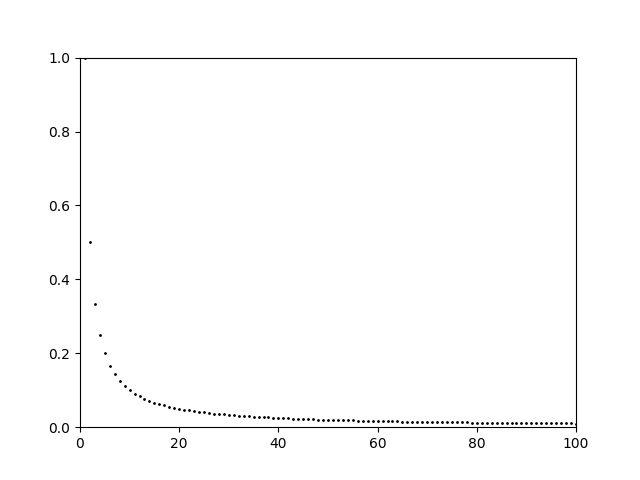
\includegraphics[width = 0.55\textwidth]{./assets/imgs/1_sur_n.png}
\caption{Les 100 premières valeurs de la suite $x_n = \frac{1}{n}$}
\label{fig:1_sur_n}
\end{figure}

Si l'on regarde le graphe de la suite, on remarque que les termes de la suite sont décroissants et qu'ils se rapprochent toujours plus de $0$ lorsque n tend vers l'infini.
On peut définir la convergence d'une suite comme suit.

On dit que les termes de la suite convergent vers une limite $l$ un réel si la distance entre $x_n$ et $l$ notée $\lvert x_n - l \rvert$ est toujours plus petit. On peut reformuler de la manière suivante :
pour toute distance $\epsilon$ aussi petite qu'on le veut, si n est suffisamment grand, alors une partie des termes de la suite seront dans l'intervalle $\lvert x_n - 0 \rvert < \epsilon$.

Désormais, imaginons qu'on considère une petite distance, par exemple $\epsilon = \frac{1}{4}$ et qu’à partir de ce $\epsilon$, on dit que les termes sont proches de la limite. Alors, il faudrait que n dépasse un certain rang N dans $\mathbb{N}$ avant qu’on ne considère que les termes soient proches.


\begin{figure}[H]
\centering 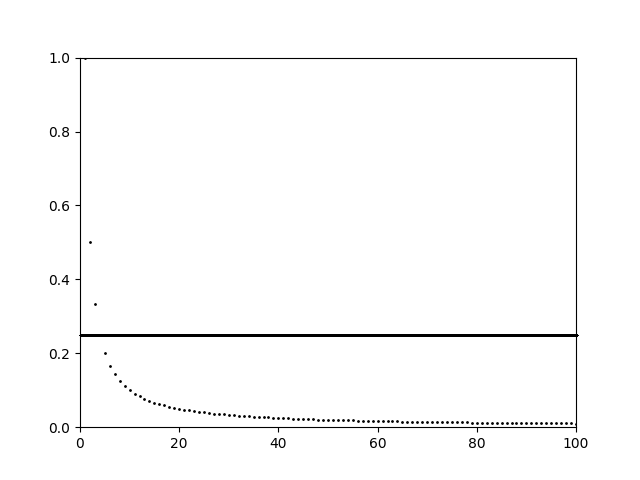
\includegraphics[width = 0.55\textwidth]{./assets/imgs/1_sur_n(1)_avec_trait.png}
\caption{Les 100 premières valeurs de la suite $x_n = \frac{1}{n}$  avec $\epsilon = \frac{1}{4}$}
\label{fig:1_sur_n_avec_trait}
\end{figure}


Mais $\frac{1}{4}$ n'est pas du tout petit et on aurait pu prendre $\frac{1}{10}$, $\frac{1}{100}$, voire $\frac{1}{1000}$, et encore plus petit. Si l’on prend par exemple $\frac{1}{100}$, alors, il faudra aussi que les termes de la suite dépassent un certain rang $n_0$ dans $\mathbb{N}$ avant qu’on ne les considère comme proches.

Mais, avec cette approche, on peut une distance très petite $\epsilon > 0$ telle que si l'on arrive à trouver un rang $n_0$ dans $\mathbb{N}$, et si pour tout les termes d'indice $n > n_0$, alors on a $\lvert x_n - l\rvert < \epsilon$.

Cela motive la définition (informelle) suivante~:

\begin{boxdef}[Convergence d'une suite (informelle)]
On dit qu'une suite $(x_n)_{n \geq 1}$ \emph{converge} vers un nombre $l \in \mathbb R$ si, en ignorant suffisamment de termes initiaux $x_1, x_2, ..., x_{n_0}$, \emph{tous} les éléments restants de la suite sont aussi proches de $l$ que l'on veut. On dit que $l$ est la \emph{limite} de la suite $(x_n)$ et on note 
\[
\lim \limits_{n \to \infty} x_n \eqdef l
\]

Si un tel nombre $l \in \mathbb R$ n'existe pas, on dit que la suite \emph{diverge}.
\label{def:convergence}
\end{boxdef}

De manière un peu plus formelle, nous aurions la définition suivante :

\begin{boxdef}[Convergence d'une suite formelle]
On dit qu'une suite numérique converge vers une limite $l$ si pour toute petite distance $\epsilon > 0$ il existe un rang $n_0$ à partir duquel les termes d'indices $n> n_0$, sont suffisemment proches de $l$ c'est-à-dire $\lvert x_n - l \rvert < \epsilon$.


Mathématiquement, la description de la définition est :

$$\forall \epsilon > 0 , \exists n_0 \in \mathbb{N} : \forall n > n_0, \lvert x_n - l \rvert < \epsilon$$

\label{def:convergence}
\end{boxdef}


Intuitivement, comme pour la suite $x_n = \frac{1}{n}$, cela signifie que lorsque $n$ est arbitrairement grand, $x_n$ devient arbitrairement proche de sa limite $l$ ($l = 0$ pour $x_n = \frac{1}{n}$). 



Reprenons à nouveau quelques exemples~:

\begin{enumerate}
    \item La suite du flocon de Koch diverge. En effet, la propriété $x_n \geq n-1$ fait qu'on s'éloigne de plus en plus de n'importe quel nombre $l \in \mathbb R$ fixé lorsque $n$ augmente.
    \item La suite $x_n = (-1)^n$ diverge. En effet, on alterne toujours entre $-1$ et $+1$, mais la suite ne se stabilise jamais sur une des deux valeurs.
    \item La suite $x_n = \frac{n+2}{n+1} = 1 + \frac{1}{n+1}$ converge vers $1$.
    \item La suite $x_n = 1$ (suite constante) converge vers $1$.
\end{enumerate}

\section{Propriétés élémentaires des limites}

Avant toute chose, et même si cela peut paraître logique, il faut quand même se poser la question~: est-ce qu'une suite convergente $(x_n)$ peut avoir deux limites distinctes $l_1 \neq l_2$ ?

La réponse est non, c'est-à-dire que

\begin{boxthm}[Unicité de la limite]
La limite d'une suite convergente est \emph{unique}.
\end{boxthm}

Raisonnons par absurde. Supposons que la suite $(x_n)$ possède deux limites $l$ et $l'$.
Par la définition de la convergence, comme la suite $(x_n)$ converge vers $l$, on a :

$$\forall \epsilon > 0 , \exists n_{0_1} \in \mathbb{N} : \forall n > n_{0_1}, \lvert x_n - l \rvert < \epsilon$$

Et comme $(x_n)$ converge aussi vers $l'$, on a :

$$\forall \epsilon > 0 , \exists n_{0_2} \in \mathbb{N} : \forall n > n_{0_2}, \lvert x_n - l' \rvert < \epsilon$$

Comme cela marche pour tout $\epsilon$, posons notre nouveau $\epsilon$ comme étant .

$$\epsilon = \frac{\lvert l-l' \rvert}{3}$$

Et posons $n_o = \max{(n_{0_1} \, , \, n_{0_2})}$.

Développons l'expression suivante.

$$\lvert l-l' \rvert = \lvert l - x_n + x_n - l'\rvert \leq \lvert  x_n - l \rvert + \lvert x_n - l'\rvert$$ 

$$\leq 2\cdot\epsilon = \frac{2\lvert l-l' \rvert}{3}$$

Ce qui est absurde, car aucun nombre ne peut être plus grand que deux tiers de lui-même. ce qui prouve bien que la limite d'une suite convergente est unique.











Il découle également de notre définition informelle que 
\begin{boxthm}[Convergence implique borné]
Toute suite convergente est bornée.
\end{boxthm}

En effet, si $(x_n)$ converge vers $l \in \mathbb R$, alors on peut séparer la suite en des termes initiaux $x_1,x_2,...,x_{n_0}$ et le reste de la suite qui est très proche de $l$, disons au moins à distance $|x_n - l| \leq 1$. Alors
$$|x_n| = |x_n - l + l| \leq |x_n - l| + |l| \leq 1 + |l| \quad \forall n \geq n_0$$ et donc
$$\min\{|x_1|, |x_2|, ..., |x_{n_0}|, l - 1\} \leq |x_n| \leq \max\{|x_1|, |x_2|, ..., |x_{n_0}|, 1 + |l|\} \quad \forall n \geq 1$$
On a alors trouvé nos deux bornes à notre suite.

Logiquement, il découle aussi le résultat suivant

\begin{boxthm}[Non-borné implique divergence]
Toute suite non-bornée est divergente.
\end{boxthm}
En effet, si une suite n'est pas bornée, alors il n'existe pas de $l$ pour appliquer la définition de la convergence :
$$\forall \epsilon > 0 , \exists n_0 \in \mathbb{N} : \forall n > n_0, \lvert x_n - l \rvert < \epsilon$$

Et donc, nous n'aurions jamais $ \lvert x_n - l \rvert < \epsilon$. Donc, la suite ne se rapproche jamais de $l$, elle s'en éloignerait toujours plus, c'est-à-dire $ \lvert x_n - l \rvert \geq \epsilon$.


En général, une suite bornée n'est pas convergente (e.g. $x_n = (-1)^n$). Cependant, si la suite est monotone (croissante ou décroissante), cela devient vrai.
\begin{boxthm}[Convergence monotone]
Toute suite bornée et monotone est convergente.
\label{thm:conv_monotone}
\end{boxthm}
Par exemple, si la suite $(x_n)$ est croissante et bornée, alors il faut se convaincre qu'on peut trouver une borne supérieure $B \in \mathbb{R}$ telle que $x_n \leq B$ pour tout $n$, et $B$. Ce $B$ agit alors comme une asymptote horizontale et la suite $(x_n)$, croissante, s'en rapproche petit à petit (cf. Figure \ref{fig:conv_monotone}).

\begin{figure}[H]
\centering 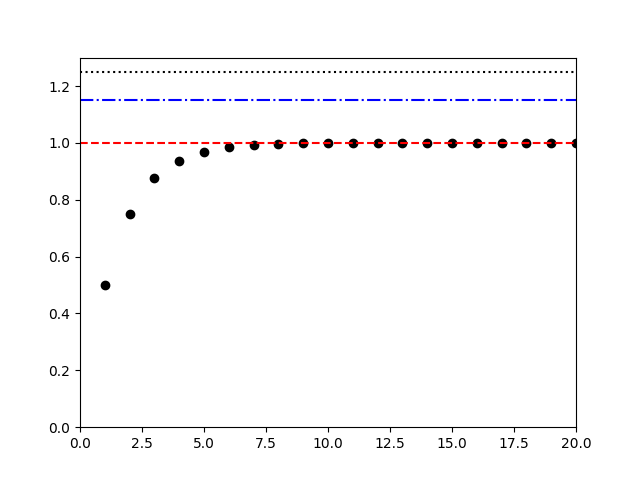
\includegraphics[width = 0.55\textwidth]{./assets/imgs/monotone_convergence.png}
\caption{Illustration de la convergence monotone avec la suite $x_n = 1 - 2^{-n}$. En rouge, on a la borne supérieure la plus petite possible ($B = 1$). En noir et bleu, on a des bornes supérieures plus grandes et donc non-optimales.}
\label{fig:conv_monotone}
\end{figure}

De manière officielle, pour prouver que la suite qui est croissante, converge vers sa borne supérieure (ici $B$),  alors on doit prouver que s'il existe un rang $n_0$ à partir duquel tous les indices $n>n_0$, alors la suite $(x_n)$ coverge vers $B$ c'est-à-dire $\lvert x_n - B \rvert < \epsilon$.


On a en développant l'inégalité :

$$-\epsilon < x_n - B < \epsilon$$

$$ B - \epsilon < x_n < B + \epsilon$$

En posant $n_0 = \lceil \max{(B-\epsilon \, , \, B + \epsilon )} \rceil$ on a trouvé effectivement ce rang $n_0$, on a donc pour tout $n>n_0$ : 

$$B-\epsilon < x_n \leq x_{n+1} \leq x_{n+2} \leq \dots < B + \epsilon$$
Et donc 

$$\lvert x_n - B \rvert < \epsilon$$
Ce qui prouve la convergence de la fonction.




Maintenant, viennent les règles de calculs sur les limites. La première est la linéarité~:

\begin{greybox}
\textbf{Linéarité de la limite.} Soit $(x_n)$ et $(y_n)$ deux suites qui convergent avec limites respectives $\lim \limits_{n \to +\infty}x_n = x$ et $\lim \limits_{n \to +\infty}y_n = y$. Soit $\lambda, \mu \in \mathbb R$ deux nombres réels. Alors la suite $(z_n) = (\lambda \cdot x_n + \mu \cdot y_n)$ converge et sa limite vaut 
$$\lim \limits_{n \to +\infty}(\lambda \cdot x_n + \mu \cdot y_n) = \lambda \cdot \left(\lim \limits_{n \to +\infty}x_n\right) + \mu \cdot \left( \lim \limits_{n \to +\infty}y_n \right) = \lambda \cdot x + \mu \cdot y$$
\end{greybox}

Pour se convaincre de ce résultat, on peut utiliser le raisonnement (informel) suivant~: Lorsque $n$ est très grand, on a $x_n \approx x$, $y_n \approx y$ et donc $\lambda \cdot x_n + \mu \cdot y_n \approx \lambda \cdot x + \mu \cdot y$.

D'une manière plus formelle (en utilisant la définition de la limite), on a :

Supposons donc qu'on a tout d'abord deux suites numériques $(x_n)$ et $(y_n)$ convergentes vers leur valeur respective $l$ et $l'$ et soient $\lambda$ et $\mu$ deux valeurs réelles non nulles (si elles étaient nulles, il n'y aurait rien à prouver). On a donc par la définition de la convergence :
pour $(x_n)$ :
$$\forall \epsilon_1 > 0 , \exists n_{0_1} \in \mathbb{N} : \forall n > n_{0_1}, \lvert x_n - l \rvert < \epsilon_1$$

Et pour $(y_n)$ :

$$\forall \epsilon_2 > 0 , \exists n_{0_2} \in \mathbb{N} : \forall n > n_{0_2}, \lvert y_n - l' \rvert < \epsilon_2$$

Pour l'addition, posons $\frac{\epsilon }{2\lvert \lambda \rvert} =\epsilon_1,$  et $\frac{\epsilon}{2\lvert \mu \rvert} = \epsilon_2$ ainsi que $n_0 = \max({n_{0_1}, n_{0_2}})$.
On peut désormais déterminer la convergence de la suite $(x_n + y_n)$ par le théorème de la convergence.

Soit notre $\epsilon$. Développons :

$$\lvert \lambda \cdot x_n + \mu \cdot y_n - (l+l') \rvert = \lvert \lambda \cdot x_n - l + \mu \cdot y_n - l' \rvert \leq \lvert \lambda \cdot x_n - l \rvert + \lvert \mu \cdot y_n - l' \rvert \leq \lvert \lambda \rvert \cdot \frac{\epsilon }{2 \lvert \lambda \rvert} + \lvert \mu \rvert \cdot \frac{\epsilon }{2 \lvert \mu \rvert} \leq \epsilon$$

Ainsi, en choisissant le rang comme N, on a donc pour tout $n>N$

$$\lvert x_n + y_n - l - l' \rvert \leq \epsilon$$


On a donc bien démontré par la convergence de la suite $(x_n + y_n)$ qui converge donc vers $l+l'$.




Le même raisonnement permet de se convaincre qu'on a le même comportement avec le produit ou quotient de deux suites convergentes.
\begin{greybox}
\textbf{Produit et quotient de limites.} Soit $(x_n)$ et $(y_n)$ deux suites qui convergent avec limites respectives $\lim \limits_{n \to +\infty}x_n = x$ et $\lim \limits_{n \to +\infty}y_n = y$. Alors~:

\begin{enumerate}
    \item La suite $(z_n) = (x_n \cdot y_n)$ converge et sa limite vaut $$\lim \limits_{n \to +\infty}(x_n \cdot y_n) = \left(\lim \limits_{n \to +\infty} x_n\right) \cdot \left(\lim \limits_{n \to +\infty} y_n\right) = x \cdot y$$
    \item Si $y,y_n \neq 0$ pour tout $n$, la suite $(z_n) = \frac{1}{y_n}$ converge et sa limite vaut $$\lim \limits_{n \to +\infty}\left( \frac{1}{y_n} \right) = \frac{1}{\lim \limits_{n \to +\infty} y_n} = \frac{1}{y}$$ 
    \item Si $y,y_n \neq 0$ pour tout $n$, la suite $(z_n) = \left(\dfrac{x_n}{y_n}\right)$ converge et sa limite vaut $$\lim \limits_{n \to +\infty}\left( \frac{x_n}{y_n} \right) = \frac{\lim \limits_{n \to +\infty} x_n}{\lim \limits_{n \to +\infty} y_n} = \frac{x}{y}$$
\end{enumerate}
\end{greybox}
Une manière formelle de montrer la multiplication est d'appliquer encore la définition de la convergence. 


Pour la multiplication, Il faut séparer deux cas : le premier est où $l = 0$, le second est où $l \ne 0$. Considérons tout d'abord le premier cas. Si $l = 0$. Nous aurions alors, avec nos deux suites $(x_n)$ et $(y_n)$ convergentes vers leur valeur respective $l$ et $l'$: 
pour $(x_n)$ :
$$\forall \epsilon_1 > 0 , \exists n_{0_1} \in \mathbb{N} : \forall n > n_{0_1}, \lvert x_n - l \rvert < \epsilon_1$$

Et pour $(y_n)$ :

$$\forall \epsilon_2 > 0 , \exists n_{0_2} \in \mathbb{N} : \forall n > n_{0_2}, \lvert y_n - l' \rvert < \epsilon_2$$


On utilise le fait que suite $(y_n)$ est convergente donc bornée (un théorème juste vu avant). Appelons $\lvert A \rvert$  la borne supérieure. Posons $\epsilon = \frac{\epsilon}{A}$ 


$$\lvert x_n \cdot y_n - l \cdot l' \rvert \leq \lvert x_n \cdot y_n  - y_n \cdot l + x_n\cdot l- l \cdot l' \rvert \leq$$

$$\lvert  y_n  \rvert \ \cdot \lvert x_n - l\rvert + \lvert l \rvert \cdot \lvert y_n - l' \rvert$$

Comme $l = 0$, on peut simplifier et on a :

$$\lvert  y_n  \rvert \ \cdot \lvert x_n - l\rvert \leq \lvert A \rvert \cdot \lvert x_n - l\rvert \leq \lvert A \rvert \cdot \frac{\epsilon}{\lvert A \rvert} \leq \epsilon$$

En choisissant le rang $n_0 = \max({n_{0_1}, n_{0_2}})$, on démontre bien la convergence.

Démontrons le deuxième cas. c'est-à-dire lorsque $l \ne 0$. On considère le même nombre $A = \max_{n>N}({\lvert v_n \rvert})$ et posons que $\frac{\epsilon}{2 \lvert A \rvert} =  \epsilon_1$ et $\frac{\epsilon}{2 \lvert l \rvert} = \epsilon_2$. On a donc :

$$\lvert x_n \cdot y_n - l \cdot l' \rvert \leq \lvert x_n \cdot y_n  - y_n \cdot l + y_n\cdot l- l \cdot l' \rvert \leq $$

$$\lvert  y_n  \rvert \ \cdot \lvert x_n - l\rvert + \lvert l \rvert \cdot \lvert y_n - l' \rvert$$

$$ \leq \lvert A \rvert \epsilon_1 + \lvert l \rvert \epsilon_2 \leq \lvert A \rvert \cdot \frac{\epsilon}{2\lvert A \rvert} + \lvert l \rvert \cdot \frac{\epsilon}{2 \lvert l \rvert} \leq 2 \cdot \frac{\epsilon}{2} \leq \epsilon $$

Ce qui démontre bien, avec la définition de la convergence que la multiplication de suites convergentes converge.

Pour l'inverse d'une suite, on applique de nouveau la convergence :

$$\forall \epsilon > 0 , \exists n_0 \in \mathbb{N} : \forall n > n_0$$ 


$$\lvert \frac{1}{y_n} - \frac{1}{l} \rvert = \lvert \frac{l-y_n}{l \cdot y_n} \rvert = \frac{\lvert l-y_n \rvert}{ \lvert l \cdot y_n \rvert} =  \frac{\lvert l-y_n \rvert}{ \lvert l \rvert \cdot \lvert y_n \rvert}$$

On a en utilisant le fait que la suite $(y_n)$ est bornée et $A$ sa borne supérieure :


$$\frac{\lvert l-y_n \rvert}{ \lvert l \rvert \cdot \lvert y_n \rvert} = \frac{\lvert l-y_n \rvert}{ \lvert l \rvert \cdot \lvert A \rvert} \leq \frac{1}{\lvert A \rvert \cdot \lvert l \rvert} \cdot \epsilon \cdot \lvert A \rvert \cdot \lvert l \rvert \leq \epsilon $$

On a donc bien montré que la suite $(y_n)$ est convergente.


Pour la troisième propriété, on utilise le fait que c'est la multiplication d'une suite et d'une inverse d'une suite. Dans ce cas, on retombe sur un cas qu'on connaît.


\section{Théorème des deux gendarmes}

Le théorème des deux gendarmes permet de déterminer la convergence d'une suite vers une limite $l \in \mathbb R$ grâce à la convergence de deux autres suites vers ce même nombre $l$.

Nous commençons par un cas particulier~:
\begin{boxthm}[Théorème des deux gendarmes : cas particulier]
Soient $(x_n)$ et $(y_n)$ deux suites et $l \in \mathbb R$. Supposons que $l \leq x_n \leq y_n$ pour tout $n$ et que la suite $(y_n)$ converge vers $l$. Alors la suite $(x_n)$ converge aussi vers $l$.
\label{thm:deux_gendarmes_part}
\end{boxthm}


La logique de ce théorème est assez similaire à celle du Théorème \ref{thm:conv_monotone} de convergence monotone. Dans le Théorème  \ref{thm:conv_monotone}, la croissance de la suite $(x_n)$ pousse la suite à converger vers la borne supérieure $B$ la plus petite. Dans notre situation, c'est la suite $(y_n)$ qui remplace la monotonie et va pousser la suite $(x_n)$ vers la borne inférieure $l$.


Du cas particulier, on peut déduire le cas général~:
\begin{boxthm}[Théorème des deux gendarmes]
Soient $(x_n)$, $(y_n)$, $(z_n)$ trois suites. Supposons que $y_n \leq x_n \leq z_n$ pour tout $n$ et que les suites $(y_n)$, $(z_n)$ convergent toutes deux vers une même limite $l \in \mathbb R$. Alors la suite $(x_n)$ converge aussi vers $l$. De manière formelle, on applique la définition de la convergence pour la suite $(y_n)$:

$$\forall \, \epsilon > 0 , \exists \, n_{0_1} \in \mathbb{N} : \forall \, n > n_{0_1}, \, \lvert y_n - l \rvert < \epsilon $$
Et
$$\forall \, \epsilon > 0 , \exists \, n_{0_2} \in \mathbb{N} : \forall \, n > n_{0_2}, \, \lvert z_n - l \rvert < \epsilon $$
Nous utilisons la première condition, c'est-à-dire pour $n > n_{0_3}$ :
$$ y_n \leq x_n \leq z_n$$
On pose $n_0 = \max{(n_{0_1} , \, n_{0_2}, \, n_{0_3})}$. Et lorsqu'on développe, pour tout $n>n_0$, on a :

$$ l-\epsilon \leq y_n \leq x_n \leq z_n \leq l+\epsilon$$

$$-\epsilon \leq y_n - l\leq x_n - l \leq z_n - l\leq \epsilon$$

C'est la définition de la convergence pour la suite $(x_n)$, donc la suite converge aussi vers la même limite $l$, avec comme rang $n_0$ ce qui est bien ce que nous voulions démontrer.
\end{boxthm}


Ici, plutôt qu'avoir une borne inférieure fixe comme dans le Théorème \ref{thm:deux_gendarmes_part}, on a une autre suite qui pousse par le bas $(x_n)$ vers la limite $l \in \mathbb R$. Étant donné que $(x_n)$ est aussi poussée par le haut vers $l$, on obtient la convergence.


Comment déduit-on rigoureusement le cas général du cas particulier ? Par hypothèse, on a l'inégalité $0 \leq x_n - y_n \leq z_n - y_n$ pour tout $n$. De plus, $(z_n - y_n)$ converge vers $0$ par linéarité de la limite. Ainsi, le cas particulier implique que $(x_n - y_n)$ converge également vers $0$. En écrivant $x_n = y_n + (x_n - y_n)$, on obtient bien que $x_n$ converge vers $l$ (à nouveau par linéarité de la limite).

Finalement, terminons par un exemple d'application. Prenons la suite $x_n = \frac{\sin(n)}{n}$ pour $n \geq 1$. On se souvient que la fonction sinus donne toujours une valeur comprise entre $-1$ et $1$. Ainsi, on déduit l'inégalité
\[
-\frac{1}{n} \leq \frac{\sin(n)}{n} \leq \frac{1}{n} \quad \forall n \in \mathbb N^*
\]
Les suites $y_n = -\frac{1}{n}$ et $z_n = \frac{1}{n}$ convergent toutes deux vers $0$, donc il en va de même pour la suite $(x_n)$ grâce au Théorème des deux gendarmes.

\section{Théorème d'un gendarme}

Lorsqu'une suite diverge, on distingue un type de divergence particulier : la divergence vers l'infini.

\begin{boxdef}[Divergence d'une suite vers l'infini (informelle)]\label{def:divergence}
On dit qu'une suite $(x_n)_{n \geq 1}$ \emph{diverge vers} $+\infty$ si, en ignorant suffisamment de termes initiaux $x_1, x_2, ..., x_{n_0}$, \emph{tous} les éléments restant de la suite sont positifs et aussi grands que l'on veut. On note 
\[
\lim \limits_{n \to \infty} x_n \eqdef +\infty
\]
Similairement, on dit qu'une suite $(x_n)_{n \geq 1}$ \emph{diverge vers} $-\infty$ si, en ignorant suffisamment de termes initiaux $x_1, x_2, ..., x_{n_0}$, \emph{tous} les éléments restant de la suite sont négatifs et aussi grands (en valeur absolue) que l'on veut. On note 
\[
\lim \limits_{n \to \infty} x_n \eqdef -\infty
\]
\end{boxdef}

Malgré la notation, il faut se rappeler qu'une telle suite ne \textbf{converge pas}. De plus, une suite non-bornée \textbf{ne diverge pas forcément vers} $\pm \infty$ (prendre l'exemple $x_n = (-1)^n \cdot n$).

Un exemple typique de suite qui diverge vers $+\infty$ est donné par $x_n = n$ (ou $x_n = -n$ pour $-\infty$). En effet, si on se donne un $B > 0$ aussi grand que l'on veut, alors à partir de l'indice $n_0 = \lceil B \rceil$, on a $x_n > 0$ et $x_n > B$ pour tous les éléments restants de la suite. En fait, n'importe quelle suite donnée par un polynôme, i.e. $x_n = P(n)$ où $P(x)$ est un polynôme réel, diverge vers $\pm \infty$.

Toutefois, le Théorème \ref{thm:deux_gendarmes_part} est aussi valable, grâce au même raisonnement, pour les suites qui divergent vers l'infini~:

\begin{boxthm}[Théorème d'un gendarme]\label{thm:un_gendarme}
Soient $(x_n)$ et $(y_n)$ deux suites. 

Supposons que $x_n \leq y_n$ pour tout $n$ et que la suite $(y_n)$ diverge vers $-\infty$. Alors la suite $(x_n)$ diverge aussi vers $-\infty$.

Similairement, supposons que $y_n \leq x_n$ pour tout $n$ et que la suite $(y_n)$ diverge vers $+\infty$. Alors la suite $(x_n)$ diverge aussi vers $+\infty$.
\end{boxthm}
De ce théorème et de l'inégalité \ref{eq:fibonacci_lower_bound}, on déduit par exemple que la suite de Fibonacci diverge vers $+\infty$.

\section{Exemples de suites typiques}
Un cas particulier de suites qui revient souvent est la suite de la forme $x_n = \frac{P(n)}{Q(n)}$ où $P(n)$ et $Q(n)$ sont deux polynômes réels et $Q(n) \neq 0$ pour tout $n$. Par exemple, on pourrait avoir les suites
$$x_n = \frac{3n+1}{7n+2}, \quad y_n = \frac{5n^5 - 2n^2 + 9}{4n^3 + 100}, \quad z_n = \frac{8n^2 + n + 1}{12n^7 - 5n^5 + 3}$$
Dans ce genre de cas, la convergence de la suite ne dépend que des termes de plus haut degré des polynômes $P(n)$ et $Q(n)$. En effet, pour $n$ grand, les autres termes sont négligeables en comparaison des termes de plus haut degré (par exemple, $n^2$ est négligeable par rapport à $n^5$). On peut alors (informellement) écrire
$$x_n \approx \frac{3n}{7n} = \frac{3}{7}, \quad y_n \approx \frac{5n^5}{4n^3} = \frac{5n^2}{4}, \quad z_n \approx \frac{8n^2}{12n^7} = \frac{2}{3n^5} \approx 0$$
et cela permet de déterminer $\lim \limits_{n \to +\infty}x_n = \frac{3}{7}$, $\lim \limits_{n \to +\infty}y_n = +\infty$ et $\lim \limits_{n \to +\infty} z_n = 0$.

Un deuxième cas de suites fréquent est la suite géométrique de la forme $x_n = r^n$ pour $r \in \mathbb R$. On peut aussi la définir par récurrence : $x_1 = 1$ et $x_{n} = r x_{n-1}$ pour $n \geq 2$. On distingue plusieurs cas

\begin{enumerate}
    \item Si $r = 1$, il s'agit de la suite constante $x_n = 1$ qui converge vers $1$.
    \item Si $r = -1$, il s'agit de la suite alternée $x_n = (-1)^n$ qui est bornée, mais diverge.
    \item Si $0 \leq r < 1$, la suite est bornée, décroissante et donc elle converge vers un certain $l \in \mathbb R$. L'équation $x_n = r x_{n-1}$ pour tout $n \geq 2$ implique que la limite doit vérifier $l = r \cdot l$, ce qui ne laisse que la possibilité $l = 0$.
    \item Si $-1 < r \leq 0$, la suite se réécrit comme $x_n = (-1)^n |r|^n$ et vérifie
    $$-|r|^n \leq x_n \leq |r|^n$$
    où $0 \leq |r| < 1$ comme dans le cas précédant. La suite converge donc vers $0$ par le théorème des deux gendarmes, mais elle n'est ni croissante, ni décroissante.
    \item Si $r > 1$, la suite diverge vers $+\infty$. Il faut penser à une "croissance exponentielle" vers $+\infty$. Pour s'en convaincre mathématiquement, on peut par exemple prouver l'inégalité de Bernoulli : $r^n \geq 1 + n(r-1)$ lorsque $r > 1$.
    \item Si $r < 1$, la suite est non-bornée et change de signe constamment. Elle diverge. 
\end{enumerate}
